\documentclass[aps,pra,reprint,amsmath,amssymb,longbibliography]{revtex4-2}
\usepackage[T1]{fontenc}
\usepackage[utf8]{inputenc}
\usepackage{graphicx}
\usepackage{booktabs}
\usepackage{bm}
\usepackage[colorlinks=true,linkcolor=blue,citecolor=blue,urlcolor=blue]{hyperref}
\newcommand{\C}{\mathbb C}
\newcommand{\E}{\mathbb E}
\newcommand{\CP}{\mathbb {CP}}
\newcommand{\Tr}{\operatorname{Tr}}
\newcommand{\Sym}{\operatorname{Sym}}
\newcommand{\End}{\operatorname{End}}
\newcommand{\ran}{\operatorname{ran}}
\newcommand{\SU}{\mathsf{SU}}
\newcommand{\PU}{\mathsf{PU}}
\newcommand{\U}{\mathsf U}
\newcommand{\ket}[1]{\lvert #1\rangle}
\newcommand{\bra}[1]{\langle #1\rvert}
\newcommand{\norm}[1]{\lVert #1\rVert}

\begin{document}
\title{Exact pure-state contraction spectrum of a three-qubit Haar circuit}
\author{Xiaojian Zeng}
\email{xiaojianzeng@foxmail.com}
\affiliation{PBC School of Finance, Tsinghua University, 100190, China}
\date{October 12, 2026}

\begin{abstract}
The slowest mode of a random quantum circuit depends on whether the circuit is tested as a distribution of unitaries or through the states it prepares. We determine the complete nonzero singular spectrum of an ordered pair of adjacent Haar-random two-qubit averages on the pure-state space of exactly three qubits. With normalized Haar measure and all constant functions removed, the sharp operator norm is $2/5$. More precisely, the principal cosines are $c_r=6/[(r+2)(2r+3)]$ for every nonnegative integer $r$, with the constant direction at $r=0$. Endpoint subgroup orbits reduce the problem to a conditional operator for single-qubit purity. Its polynomial filtration and a Haar-frame radial law yield a complete Jacobi-polynomial diagonalization. A unitary coherent-symbol construction then transfers the spectrum to conjugation on $\End(\Sym^k\C^8)$, where it truncates at $r=\lfloor k/2\rfloor$. Thus no higher symmetric state moment introduces a slower mode than centered purity. For $m$ ordered layer pairs the exact stationary square-integrable contraction is $(2/5)^{2m-1}$. The familiar second-moment value is recovered, while the universal all-representation three-qubit unitary-group constant remains unresolved. The result concerns square-integrable observables and densities relative to stationary Haar measure, without a total-variation assertion for a deterministic initial state.
\end{abstract}
\maketitle

\section{Introduction}

Random quantum circuits are used to prepare typical states and to approximate Haar-random unitary transformations. These tasks test different representation families. Spectral gaps for local circuits have been studied through moment Hamiltonians, three-site operators, and comparisons between circuit architectures \cite{Haferkamp2021,Allen2025,Deneris2025}. Even on three qubits, knowing a low moment does not determine the slowest mode in every representation of the unitary group.

Dong and Fan \cite{Dong2026} formulate the all-representation problem for adjacent Haar-$\SU(4)$ gates. Their exact witness in $\End(\bigwedge^4\C^8)$ gives a nonfixed principal cosine $1/2$, while the matching universal upper bound remains open in the checked version. The second-moment value $2/5$, equivalently a two-edge moment-Hamiltonian gap $3/5$, is already present in earlier work \cite{Haferkamp2021}. Our purpose is to determine the complete spectrum for the natural pure-state quotient and every symmetric state-moment order of this same circuit.

The stationary probability inputs have substantial prior history. Induced measures give the one-qubit purity distribution \cite{Zyczkowski2001,Enriquez2018}; complex Haar corners have an explicit matrix-ball law \cite{Fyodorov2007}; and the full joint distribution of the three one-qubit spectra is known \cite{Christandl2014}. We do not claim a new stationary density or a new general moment-integration method. The calculation below turns those inputs into an explicit diagonalization of the local-circuit conditional operator, with a complete dynamical spectrum, a sharp ordered-power norm, and a transfer preserving the physical Hilbert--Schmidt metric. The contribution is the all-degree spectrum and its dynamical consequences, rather than the previously known number $2/5$.

\section{Model and exact result}
\label{sec:model}

Let $\mathcal H=(\C^2)^{\otimes3}=\C^8$ and let $\mu$ be normalized Haar, or Fubini--Study, probability on $\CP^7$. We use the unitary representation
\begin{equation}
 (\mathcal U(g)f)(\psi)=f(g^{-1}\psi)
\end{equation}
on $L^2(\CP^7,\mu)$. The local groups act as $\SU(4)$ on qubits $12$ or $23$, with the identity on the spectator. Their normalized Haar averages are orthogonal projections $Q_{12}$ and $Q_{23}$. Write
\begin{equation}
 M=Q_{12}Q_{23},\qquad Af=\int f\,d\mu.
\label{eq:M}
\end{equation}
The reverse ordering is $M^*$ and has the same norms. Time is measured in independent pairs of adjacent gates; all norms, cosines, and gaps are dimensionless. There are exactly three sites, complex Haar gates, open adjacent edges, and no noise, approximation, or thermodynamic limit.

For a normalized state define the endpoint statistics
\begin{equation}
 \rho_i=\Tr_{\{1,2,3\}\setminus\{i\}}\ket\psi\bra\psi,
 \quad t_i=2\Tr\rho_i^2-1=|\bm b_i|^2,
\label{eq:t}
\end{equation}
where $\rho_i=(I+\bm b_i\cdot\bm\sigma)/2$. Thus $0\leq t_i\leq1$. Their common stationary density is
\begin{equation}
 w(t)=\frac{105}{16}\,t^{1/2}(1-t)^2,\qquad 0<t<1.
\label{eq:weight}
\end{equation}
Let $p_r$ be real orthonormal polynomials for this probability density, of degree $r$, with $p_0=1$. They are normalized multiples of $P_r^{(2,1/2)}(2t-1)$.

\textbf{Exact spectrum.} The complete nonzero singular values of $M$ are simple and equal to
\begin{equation}
 c_r=\frac{6}{(r+2)(2r+3)},\qquad r=0,1,2,\ldots .
\label{eq:spectrum}
\end{equation}
The value $c_0=1$ is precisely the constant direction. In particular,
\begin{align}
 \norm{M-A}&=\frac25,\nonumber\\
 \norm{M^m-A}&=\left(\frac25\right)^{2m-1},\quad m\geq1.
\label{eq:powers}
\end{align}
In conjugation on $\End(\Sym^k\C^8)$, equipped with the Hilbert--Schmidt metric, the same singular values truncate to $0\leq r\leq\lfloor k/2\rfloor$. Removing the entire global invariant gives
\begin{equation}
 \norm{Q_{12}^{(k)}Q_{23}^{(k)}-A_k}
 =\begin{cases}0,&k=0,1,\\[2pt]2/5,&k\geq2,\end{cases}
\label{eq:finite}
\end{equation}
where $A_k(X)=\Tr(X)I/\dim(\Sym^k\C^8)$. Here $k$ is the symmetric state-moment order, not the number of physical qubits.

The proof has three ingredients: complete endpoint orbit reduction, the all-degree conditional spectrum, and a unitary transfer to finite moments. None of the infinite quantifiers is inferred from a finite spectral scan.

\section{Endpoint orbits and conditional purity}
\label{sec:orbits}

\subsection{Completion preserves the gate product}

Let $X_3$ and $Y_1$ be the one-qubit Haar-$\SU(2)$ averages on spectators $3$ and $1$, respectively, and set
\begin{equation}
 P_3=Q_{12}X_3,\qquad P_1=Q_{23}Y_1.
\end{equation}
Each is an orthogonal projection because its two factors commute. Spectator group inclusion implies $X_3Q_{23}=Q_{23}$ and $Q_{12}Y_1=Q_{12}$. Consequently
\begin{equation}
 P_3P_1=Q_{12}X_3Q_{23}Y_1=Q_{12}Q_{23}=M.
\label{eq:completion}
\end{equation}
This identity is the spectator-completion lemma of Dong and Fan \cite{Dong2026}. It applies in any unitary representation. We rederive it to emphasize that completing the endpoint orbits preserves the operator itself; no nonzero mode is removed by assumption.

\subsection{The complete invariant statistic}

The orbit of $\SU(4)$ on the two-qubit complement and $\SU(2)$ on the spectator is classified by the two Schmidt eigenvalues of the spectator. A fixed reduced matrix has purifications related by a unitary on $\C^4$, and the spectator group rotates its eigenbasis. Requiring determinant one on $\C^4$ introduces no additional invariant: the purification occupies at most two dimensions, so a unitary on the unused complement can correct the determinant while leaving the state unchanged. On projective pure states the orbit is therefore specified completely by $t_i$.

It follows, including the degenerate spectra up to measure-zero strata, that
\begin{equation}
 \ran P_i=\{f(t_i):f\in L^2([0,1],w(t)\,dt)\},\quad i=1,3.
\label{eq:range}
\end{equation}
The density in Eq.~\eqref{eq:weight} follows by transforming the established $2\times4$ induced eigenvalue law, proportional to
$(\lambda_+-\lambda_-)^2\lambda_+^2\lambda_-^2\delta(1-\lambda_+-\lambda_-)$, under $t=(\lambda_+-\lambda_-)^2$ \cite{Zyczkowski2001,Enriquez2018}. It integrates to one and has mean $\E t=1/3$.

Define isometries $J_i f=f(t_i)$. The cross operator
\begin{equation}
 T=J_1^*J_3,\qquad (Tf)(x)=\E[f(t_3)\mid t_1=x]
\label{eq:T}
\end{equation}
is a contraction. Endpoint exchange symmetry of Haar measure makes it self-adjoint on $L^2(w)$. In particular $J_3^*J_1=T$ also, and
\begin{equation}
 M=J_3TJ_1^*.
\label{eq:factor}
\end{equation}
The reduction keeps the full joint law. The known three-qubit joint marginal distribution \cite{Christandl2014} could also be used to construct $T$; the following frame calculation avoids integrating its piecewise density.

\subsection{Polynomial filtration at every degree}

Fix $t_1=x=d^2$ and Schmidt weights $\lambda_\pm=(1\pm d)/2$. In a Schmidt basis on qubit $1$, the complementary vectors $u,v\in\C^4$ form a Haar orthonormal two-frame, conditional on these weights. Let $\bm a$ and $\bm b$ be their reduced Bloch vectors on qubit $3$. Then
\begin{equation}
 \bm b_3=\frac{\bm a+\bm b}{2}
              +d\frac{\bm a-\bm b}{2}.
\label{eq:frame}
\end{equation}
For any integer $r\geq0$, $t_3^r$ is a polynomial in $d$ of degree at most $2r$. The frame law is invariant under exchanging its columns. This exchange reverses the second term of Eq.~\eqref{eq:frame}, so averaging eliminates every odd power of $d$. Therefore
\begin{equation}
 T(t^r)\ \hbox{has degree at most }r,
\end{equation}
and its coefficient of $x^r$ is
\begin{equation}
 m_r=\E R^{2r},\qquad R=\frac{|\bm a-\bm b|}{2}.
\label{eq:leading}
\end{equation}
This is a finite polynomial argument for arbitrary $r$, independent of the moment tables below.

\section{The full conditional spectrum}
\label{sec:conditional}

\subsection{An exact Haar-frame radial law}

Put $V=(u,v)$ and let $P$ be the rank-two projector onto the qubit-$3$ computational-zero subspace of $\C^4$. The Hermitian matrix
\begin{equation}
 B=V^*PV
\end{equation}
is uniform in Cartesian Hermitian volume on $0<B<I$. This is the $N=4$, square $2\times2$ specialization of the complex Haar-corner law \cite{Fyodorov2007}. For clarity, it also follows directly from normalized Gaussian frames.

Partition a standard complex Gaussian $4\times2$ matrix $G$ into square blocks $G_1,G_2$. With $W_j=G_j^*G_j$ and $S=W_1+W_2$, the frame $V=GS^{-1/2}$ is Haar by unitary invariance. Square complex polar integration gives independent densities proportional to $e^{-\Tr W_j}\,dW_j$. At fixed $S$, the change of variables
\begin{equation}
 W_1=S^{1/2}BS^{1/2},\qquad W_2=S-W_1
\end{equation}
has Hermitian Jacobian $(\det S)^2$. Indeed, when $S$ is diagonal its two diagonal coordinates scale by $s_1,s_2$, and the two real off-diagonal coordinates by $\sqrt{s_1s_2}$ each. Thus the joint density factors as
\begin{equation}
 \text{const.}\ e^{-\Tr S}(\det S)^2\,dS\,dB,
 \qquad S>0,\quad 0<B<I.
\end{equation}
Integrating $S$ proves the stated uniform law for $B$.

Writing its unordered eigenvalues as $s_1,s_2$, the complex Hermitian Jacobian gives
\begin{equation}
 p(s_1,s_2)=6(s_1-s_2)^2,\qquad 0<s_1,s_2<1,
\end{equation}
with independent Haar eigenvectors. Hence $\delta=|s_1-s_2|$ has density $12\delta^2(1-\delta)$. A Haar eigenbasis in two dimensions implies that $B_{11}-B_{22}$, conditional on $\delta$, is uniform on $[-\delta,\delta]$.

In the original frame variables this difference is the $z$ component of $(\bm a-\bm b)/2$:
\begin{equation}
 z=\frac{a_z-b_z}{2}=u^*Pu-v^*Pv=B_{11}-B_{22}.
\end{equation}
Integrating the conditional uniform density yields
\begin{equation}
 p_z(z)=1-3z^2+2|z|^3,\qquad |z|<1.
\label{eq:component}
\end{equation}
Spectator rotations make the three-vector $(\bm a-\bm b)/2$ isotropic. Its component density consequently satisfies
\begin{equation}
 p_z(z)=\int_{|z|}^1\frac{p_R(R)}{2R}\,dR.
\end{equation}
Differentiating Eq.~\eqref{eq:component} gives
\begin{equation}
 p_R(R)=12R^2(1-R),\qquad 0<R<1.
\label{eq:radial}
\end{equation}
This integrates to one, leaving no atom at zero or at an endpoint. The identification of the component law and isotropic radial law is essential; the eigenvalue gap of $B$ was not assumed to be the original Bloch-vector radius.

Combining Eqs.~\eqref{eq:leading} and \eqref{eq:radial}, for every $r\geq0$,
\begin{align}
 m_r&=12\int_0^1 R^{2r+2}(1-R)\,dR\nonumber\\
    &=\frac{12}{(2r+3)(2r+4)}
     =\frac{6}{(r+2)(2r+3)}.
\label{eq:mr}
\end{align}
The derivation uses complex Haar frames in $\C^4$ and a rank-two projector. It does not apply unchanged to real gates, other local dimensions, or non-Haar ensembles.

\subsection{Complete Jacobi diagonalization}

Polynomial preservation gives $Tp_r$ degree at most $r$. For each polynomial $q$ of lower degree, self-adjointness gives
\begin{equation}
 \langle Tp_r,q\rangle_w=\langle p_r,Tq\rangle_w=0.
\end{equation}
Thus $Tp_r$ is a multiple of $p_r$. Comparing leading coefficients using Eq.~\eqref{eq:mr} gives
\begin{equation}
 Tp_r=c_rp_r.
\label{eq:diagonal}
\end{equation}
Polynomials are dense in $L^2(w)$: continuous functions are dense for this finite measure, and polynomials uniformly approximate continuous functions on $[0,1]$. Equation~\eqref{eq:diagonal} is therefore the complete diagonalization, not an ansatz restricted to polynomials. The positive sequence $c_r$ decreases strictly from $1$ to $0$. In particular $T$ is compact, and the norm of its tail beyond degree $L$ is exactly $c_{L+1}$.

Writing $e_{i,r}=J_ip_r$, the two orthonormal endpoint families obey
\begin{equation}
 \langle e_{1,r},e_{3,s}\rangle=c_r\delta_{rs}.
\end{equation}
Equation~\eqref{eq:factor} then has the singular expansion
\begin{equation}
 M=\sum_{r\geq0}c_r\ket{e_{3,r}}\bra{e_{1,r}}.
\label{eq:svd}
\end{equation}
Components orthogonal to $\ran P_1$ map to zero. The term $r=0$ is the constant projection $A$. This proves the complete spectrum and the first norm in Eq.~\eqref{eq:powers}. Its sharp mode is centered one-qubit purity, since $p_1$ is proportional to $t-1/3$.

The ordered-power exponent follows from the overlap of the two endpoint families, not from raising singular values directly to the $m$th power:
\begin{equation}
 M^m-A=\sum_{r\geq1}c_r^{2m-1}
              \ket{e_{3,r}}\bra{e_{1,r}}.
\label{eq:mpower}
\end{equation}
Taking its norm proves Eq.~\eqref{eq:powers}. The nonconstant spectral radius of $M$ is $c_1^2=4/25$, distinct from the one-pair norm $2/5$.

\section{All symmetric state moments}
\label{sec:finite}

Let $W_k=\Sym^k\C^8$. Its conjugation representation on $\End(W_k)$ is center-trivial, so it descends to $\PU(8)$. Equip it with the physical Hilbert--Schmidt inner product and define the coherent symbol
\begin{equation}
 (S_kX)(\psi)=\langle\psi^{\otimes k},X\psi^{\otimes k}\rangle.
\label{eq:symbol}
\end{equation}
This is an equivariant map to $L^2(\CP^7,\mu)$, with image $\mathcal V_k$ consisting of restrictions of homogeneous polynomials of bidegree $(k,k)$. It is injective. Vanishing on all unit vectors implies vanishing on all complex vectors by homogeneity, and independence of the holomorphic and antiholomorphic monomials forces every operator coefficient to vanish.

The symbol itself need not be an isometry. Instead set $D_k=S_k^*S_k$, a positive definite operator commuting with the global $\SU(8)$ action. Then
\begin{equation}
 U_k=S_kD_k^{-1/2}
\label{eq:unitary}
\end{equation}
is a unitary intertwiner onto $\mathcal V_k$. This step transfers local projection angles in the Hilbert--Schmidt metric, rather than in an arbitrary Euclidean metric for polynomial coefficients.

The completed endpoint subgroup has the multiplicity-free Cauchy branching
\begin{equation}
 W_k\big|_{\SU(4)\times\SU(2)}
 =\bigoplus_{j=0}^{\lfloor k/2\rfloor}
 S_{(k-j,j)}\C^4\otimes S_{(k-j,j)}\C^2,
\label{eq:branch}
\end{equation}
where $S_\lambda$ denotes the Schur functor. The summands are distinct, so the completed conjugation commutant has dimension $\lfloor k/2\rfloor+1$.

For each $j\leq\lfloor k/2\rfloor$, $t_i^j$ belongs to $\mathcal V_k$. To see its degree explicitly, extend $\rho_i$ to the unnormalized reduced matrix $\widetilde\rho_i$ of an arbitrary vector. The polynomial
\begin{equation}
 \left(2\Tr\widetilde\rho_i^2-\norm\psi^4\right)^j
                  \norm\psi^{2(k-2j)}
\end{equation}
has bidegree $(k,k)$ and restricts to $t_i^j$ on the unit sphere. These independent invariant symbols already match the full commutant dimension. Consequently
\begin{equation}
 \mathcal V_k\cap\ran P_i
 =\operatorname{span}\{p_0(t_i),\ldots,p_{\lfloor k/2\rfloor}(t_i)\}.
\end{equation}
Restricting Eq.~\eqref{eq:svd} to $\mathcal V_k$ proves the truncated spectrum in the physical metric through Eq.~\eqref{eq:unitary}.

Finally $W_k$ is globally irreducible, so its entire global commutant is the identity line. For $k=0,1$ only $r=0$ survives; for every $k\geq2$, $r=1$ is present and is strictly the largest nonconstant angle. This proves Eq.~\eqref{eq:finite} at all integer orders.

\section{Exact checks and physical scope}
\label{sec:scope}

Two finite reconstructions support the analytic result. The first constructs endpoint Lie generators as bosonic differential operators $x_a\partial_b$ in the occupation basis. The second constructs spectator Casimirs from symmetrized tensor-slot swaps, with a different mode ordering and rational row algebra. Both use the factorial monomial metric, test complete sector projections, match all cross-Gram entries exactly, and subtract the full identity direction. Their shared model and prior derivation mean these are different computational representations, not independent external peer review.

The spaces have dimensions $\dim W_7=3432$ and $\dim W_8=6435$. The corresponding sector ranks and complete nonfixed angles are shown in Table~\ref{tab:checks}. The degree-eight calculation includes the additional angle $c_4=1/11$ predicted by the formula. These finite data check conventions and omitted-invariant errors; the all-degree argument in Secs.~\ref{sec:conditional} and \ref{sec:finite} supplies the infinite coverage. No floating-point eigensolver or fitted rational reconstruction enters the proof.

\begin{table}[tb]
\caption{Exact supporting calculations in the symmetric representation family. The ranks are the completed endpoint sector dimensions in $W_k$; the constant singular value $1$ is omitted from the last column.}
\label{tab:checks}
\begin{ruledtabular}
\begin{tabular}{ccl}
$k$ & Sector ranks & Nonfixed angles\\
\hline
7 & $960,1296,896,280$ & $2/5,\ 3/14,\ 2/15$\\
8 & $1485,2205,1800,840,105$ & $2/5,\ 3/14,\ 2/15,\ 1/11$
\end{tabular}
\end{ruledtabular}
\end{table}

\begin{figure}[tb]
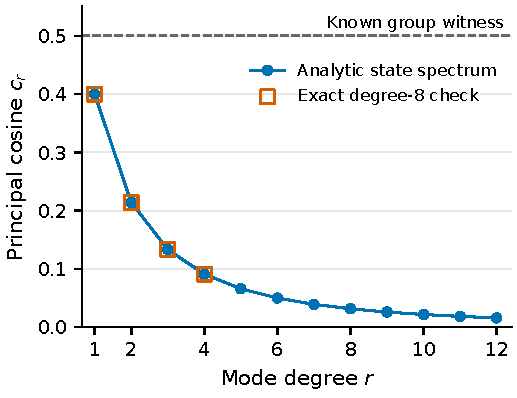
\includegraphics[width=\columnwidth]{figures/spectrum.pdf}
\caption{Nonconstant analytic principal cosines, Eq.~\eqref{eq:spectrum}, with the constant $c_0=1$ removed. Squares mark the exact degree-eight values. The dashed line is the known $1/2$ witness in a different, fourth-exterior-power representation \cite{Dong2026}; it is not an upper bound on every unitary-group mode. The plot is generated from exact rational data by AI-assisted Python/Matplotlib code and contains no sampled experimental data.}
\label{fig:spectrum}
\end{figure}

As low-degree checks, conditional expectations from the diagonalization are
\begin{align}
 \E[t_3\mid t_1=t]&=\frac15+\frac25t,\nonumber\\
 \E[t_3^2\mid t_1=t]&=\frac1{14}+\frac17t+\frac3{14}t^2.
\end{align}
Both identities follow by expanding in the first three Jacobi polynomials and are checked by the supplied exact-algebra program. The first relation exhibits the slowest centered mode directly. Figure~\ref{fig:spectrum} displays the faster added modes.

The contraction applies to square-integrable state observables and state densities relative to $\mu$. For such $f$, Eq.~\eqref{eq:powers} gives
\begin{equation}
 \norm{M^mf-Af}_{L^2(\mu)}
 \leq\left(\frac25\right)^{2m-1}\norm{f-Af}_{L^2(\mu)},
\end{equation}
with the same sharp norm for densities under the adjoint ordering. A deterministic initial state defines a delta measure, which is outside this $L^2$ domain. No total-variation mixing time from that initial law is established here.

The result distinguishes several conventions. On the pure-state quotient the two-projector Hamiltonian $(I-Q_{12})+(I-Q_{23})$ has gap $1-c_1=3/5$, while the equally weighted random-edge mean has gap $(1-c_1)/2=3/10$. These follow from the principal-angle blocks of the raw projections, whose nonzero angles are preserved by Eq.~\eqref{eq:completion}. They are not the nonnormal product spectral radius $4/25$ or its singular norm $2/5$.

The family $\End(\Sym^k\C^8)$ is physically natural for symmetric state moments, but it does not exhaust all representations of $\PU(8)$. In particular, the established fourth-exterior-power $1/2$ mode is absent. We therefore obtain no matching universal upper bound for the original constant
\begin{equation}
 c_* =\sup_{\rho}\norm{Q_{12}(\rho)Q_{23}(\rho)-A(\rho)},
\end{equation}
where $\rho$ ranges over finite-dimensional continuous unitary representations of $\PU(8)$. Whether $c_*=1/2$ remains unresolved in the checked primary literature \cite{Dong2026}. Our exact state-quotient sequence rules out slower modes at arbitrarily high symmetric order, without settling that larger unitary-design problem. Priority screening for the complete sequence is bounded; no claim of an exhaustive literature exclusion is made.

\section*{Research methods and AI disclosure}

OpenAI Codex systems were used substantively for literature comparison, development of the analytic argument, exact calculation and code generation, automated checking in separate sessions, figure code, and preparation of this manuscript. The supporting calculations use arbitrary-precision integer and rational arithmetic with Python and SymPy; the figure uses Matplotlib only for rendering exact values. Automated checks supplement the displayed derivation and do not constitute external peer review. Human scientific verification and confirmation of responsibility for this local draft remain pending. The detailed tools and reproduction instructions accompany the manuscript.

\bigskip
\section*{Data availability}

The exact supporting inputs, calculation programs, rational spectrum data, and regeneration instructions are included in the accompanying local reproducibility package. No experimental dataset is used. No public data repository deposit is claimed.

\bibliography{references}
\end{document}
